% Copyright 2004 by Till Tantau <tantau@users.sourceforge.net>.

\documentclass{beamer}
\usepackage{amsmath, amsthm, amssymb}
\usepackage{graphicx}
\usepackage{float}
\usepackage{tikz}
\usepackage{pifont}
\usepackage{color}
\usepackage[font = footnotesize]{subcaption}
\usepackage[backend=bibtex, bibstyle = numeric, citestyle=numeric, maxnames = 4, minnames = 1]{biblatex}
\addbibresource{ref.bib}

\newcommand{\cmark}{\ding{51}}
\newcommand{\xmark}{\ding{55}}

\usetikzlibrary{shapes.geometric, arrows}

\tikzstyle{input} = [rectangle, rounded corners, minimum width = 3cm,
minimum height = 1cm, text centered, draw = black, fill = red!30]
\tikzstyle{arrow} = [thick, ->, >=stealth]

\usetheme{CambridgeUS}


\title{Automated Summarisation of Big Data}
\subtitle{Using data from the Catlin Seaview Survey - a global coral reef monitoring effort}
\author{Amy StringeR}
\institute[Global Change Institute]
{
  \inst{1}%
  University of Queensland
}
\date{August 2018}

% Add logo
\pgfdeclareimage[height=0.5cm]{university-logo}{logos}
\logo{\pgfuseimage{university-logo}}


% Let's get started
\begin{document}
    \section{IntRoduction}
        \begin{frame}
          \titlepage
        \end{frame}

        \begin{frame}{Outline}
          \tableofcontents
        \end{frame}

% Section and subsections will appear in the presentation overview
% and table of contents.
    \section{Context}
        \begin{frame}{The Catlin Seaview Survey}
          \begin{columns}[T]
            \begin{column}{0.45\textwidth}
              \begin{itemize}
                \item Aim to develop a global baseline on reef health and then monitor the state of these reefs through resurvey efforts
                \item 5 regions around the world so far: The Great Barrier Reef, the Caribbean, Southeast Asia, the Indian Ocean, The Pacific
                  \begin{itemize}
                    \item a total of 25 survey countries
                  \end{itemize}
              \end{itemize}
            \end{column}

            \begin{column}{0.45\textwidth}
              \vskip-\baselineskip
                \begin{figure}
                  \centering
                      \begin{subfigure}[t]{0.6\textwidth}
                        \centering
                        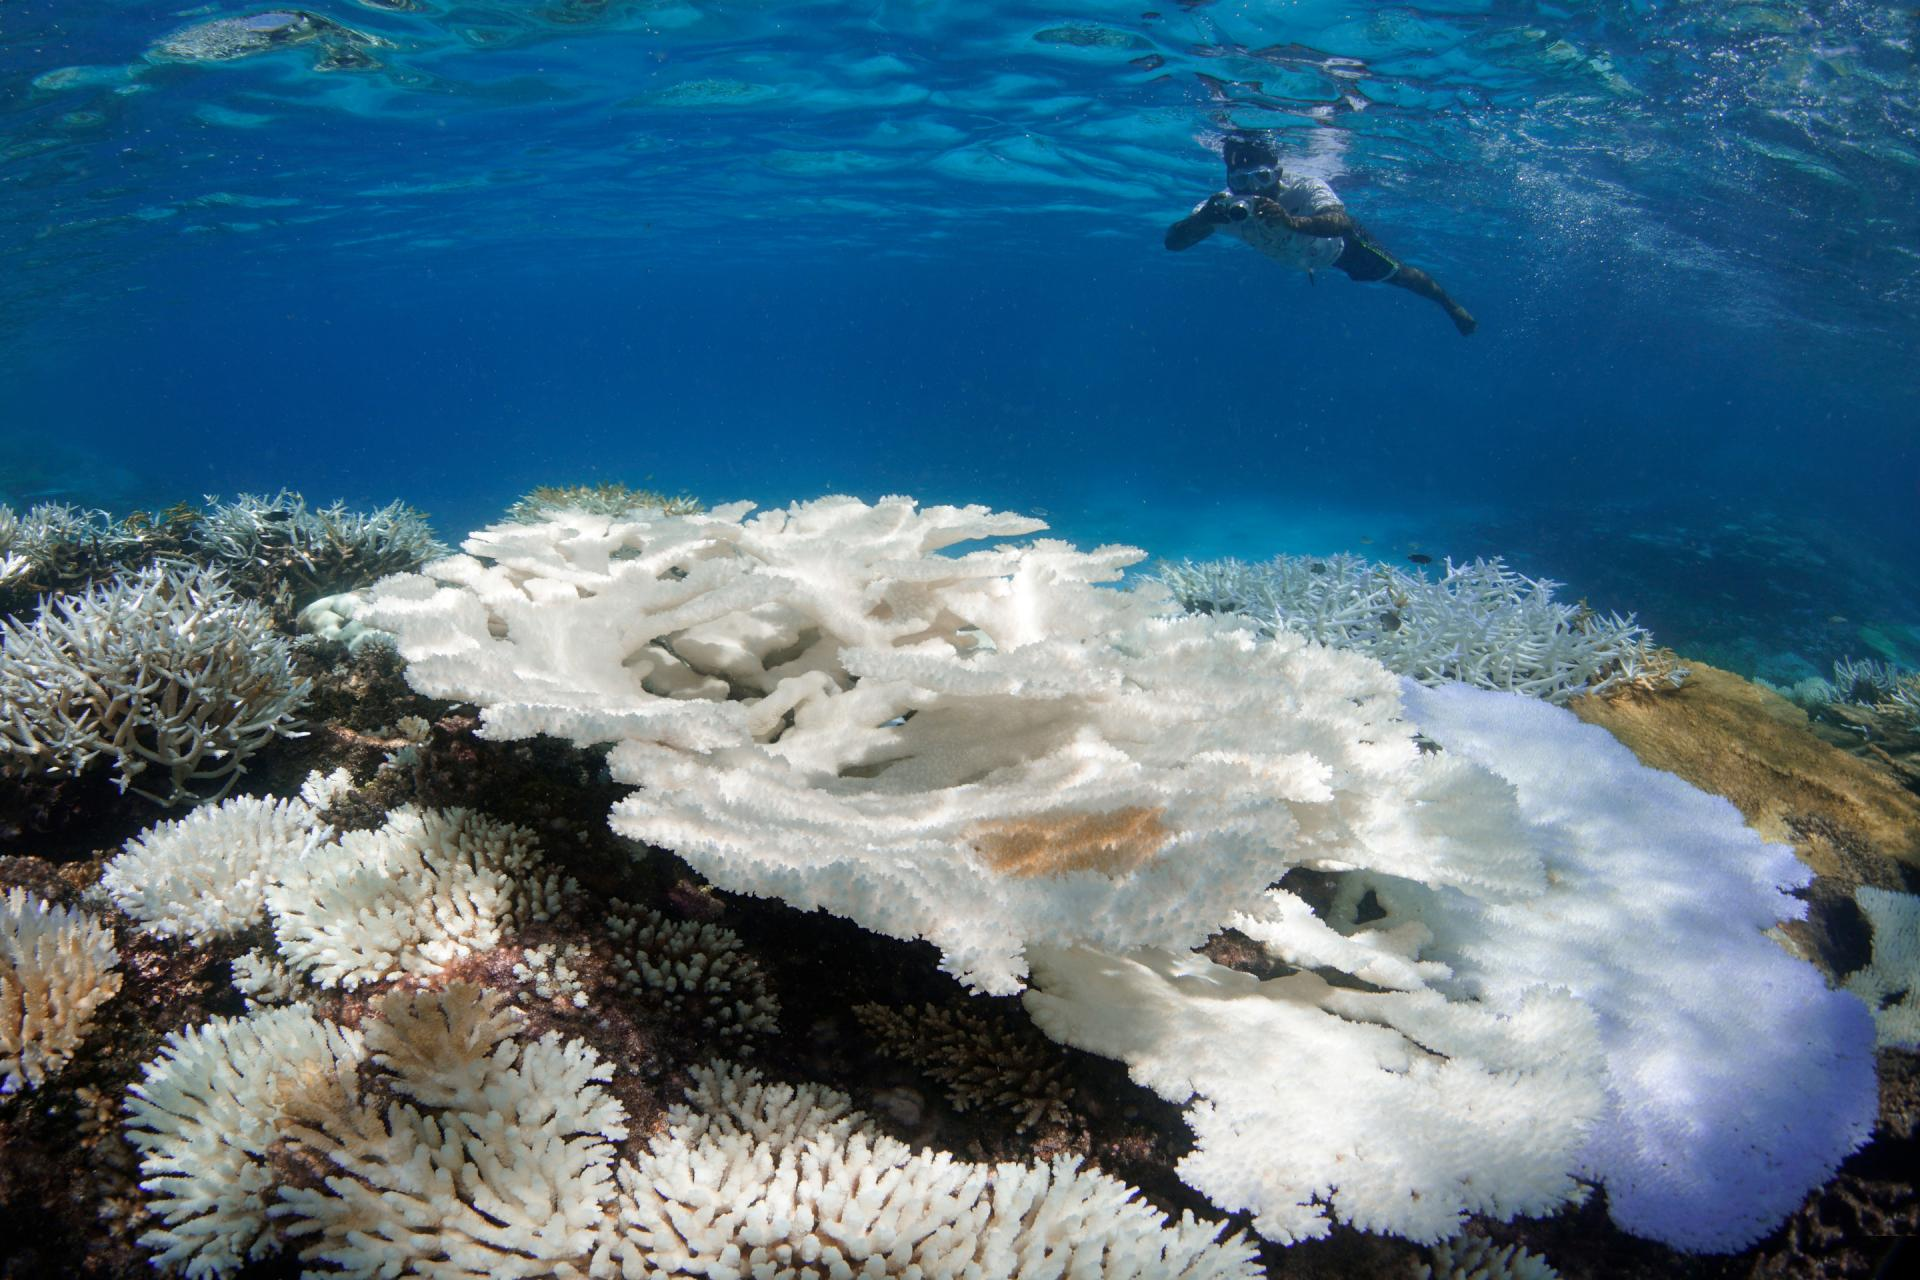
\includegraphics[width = \linewidth]{bleach1_maldives.jpeg}
                        \caption{Bleaching at the Maldives, 2016}
                        \label{fig:bleach_maldives}
                      \end{subfigure} \hskip 1em%
                      \begin{subfigure}[t]{0.6\textwidth}
                        \centering
                        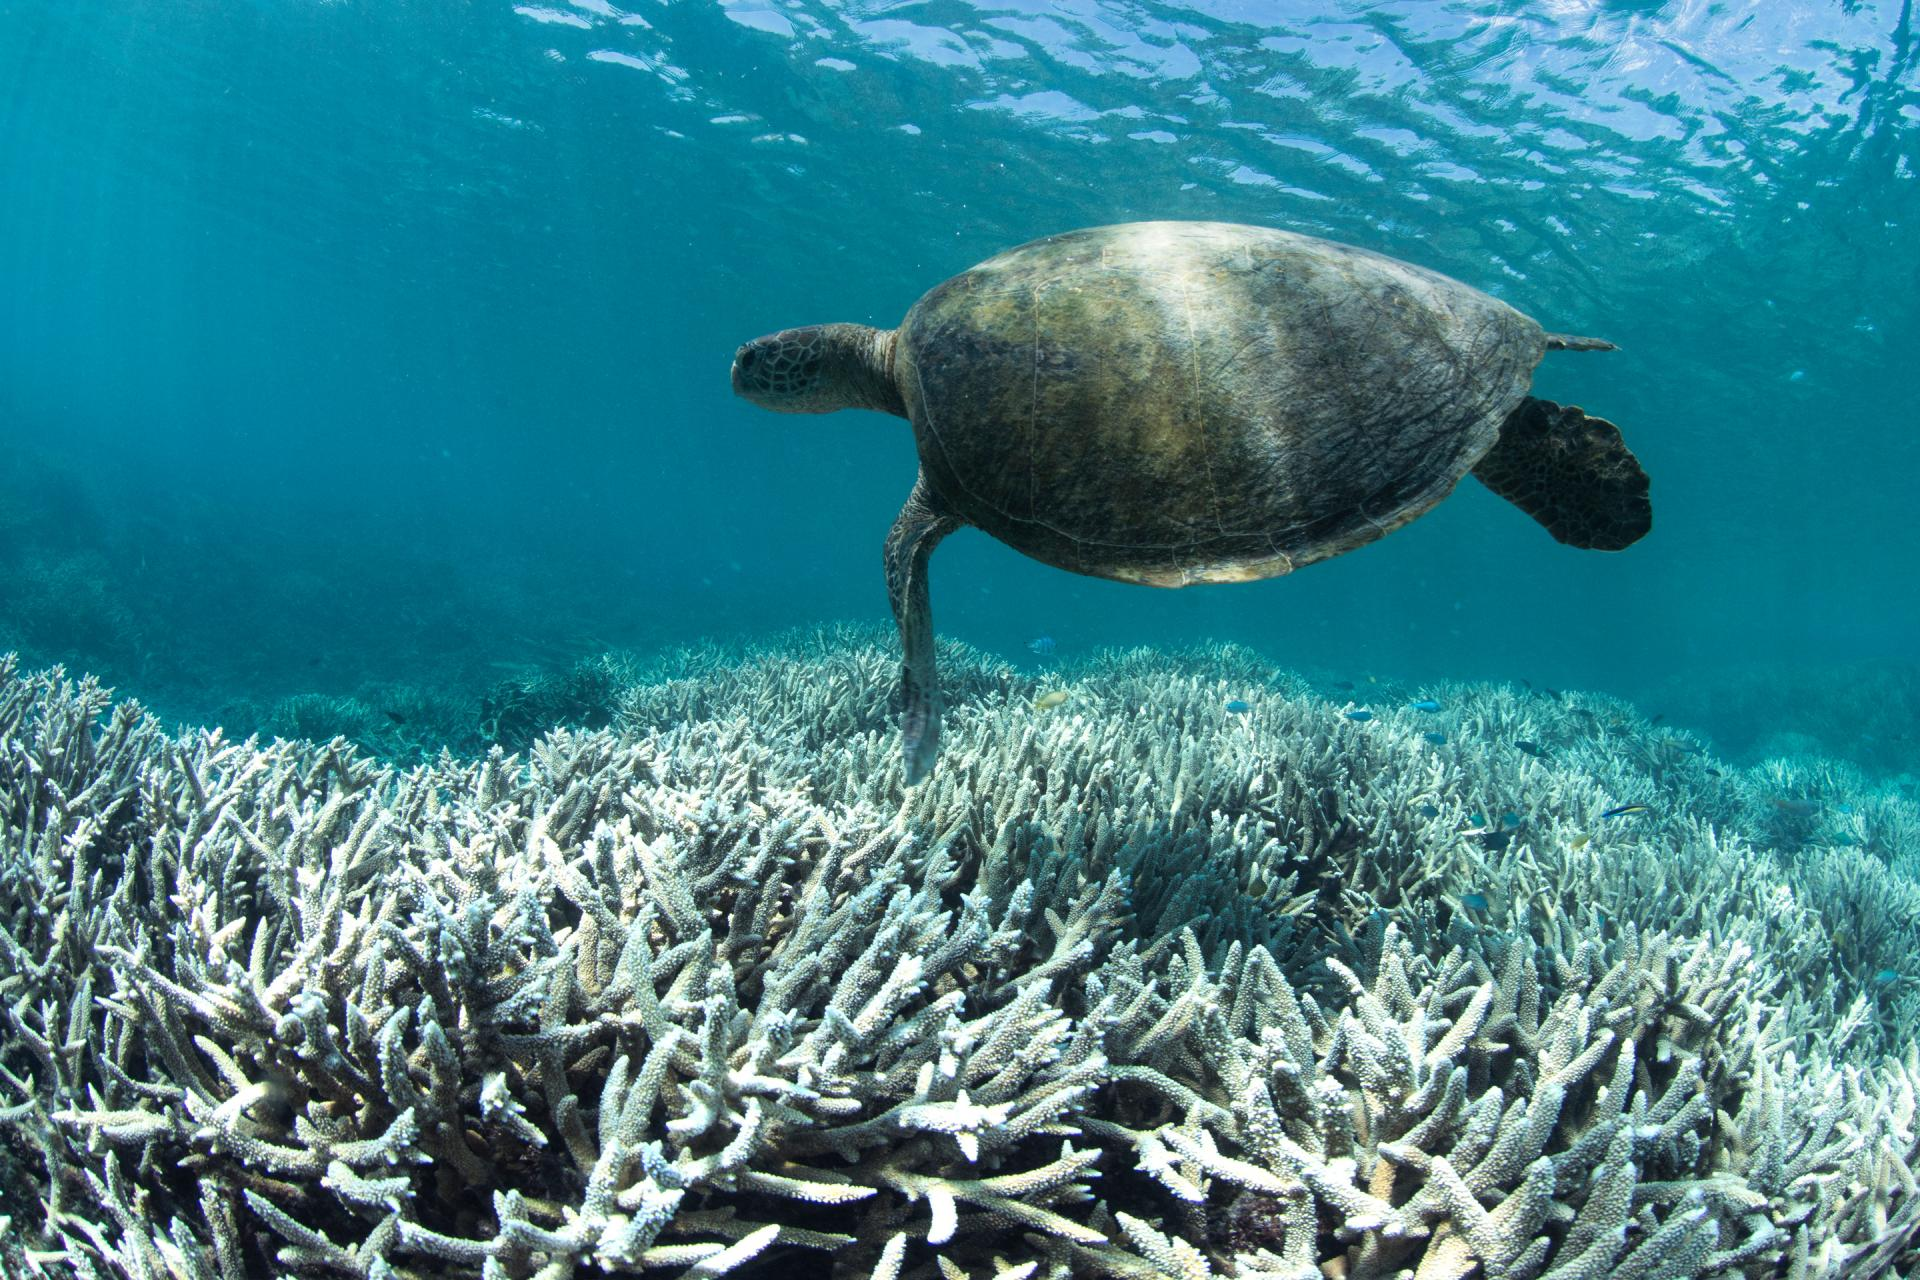
\includegraphics[width = \linewidth]{bleach3_heron.jpeg}
                        \caption{Bleaching at Heron Island, 2016}
                        \label{fig:bleach_heron}
                      \end{subfigure}
                \end{figure}
            \end{column}
          \end{columns}
        \end{frame}

        \subsection{The Catlin Data}
            \begin{frame}{Efficient Monitoring}
                Three main stages:
                  \begin{enumerate}
                    \item Collection of images
                    \item Annotation of images
                    \item Calculating proportions, and visualising trends between surveys
                  \end{enumerate}
            \end{frame}

        \subsection{Image Collection}
            \begin{frame}{The Catlin Seaview Survey - Image Collection }
              \begin{columns}[T]
                \begin{column}{0.48\textwidth}
                  \centering
                  \begin{itemize}
                    \item HD images collected in 2km transects along a reef section - taken automatically every 3 seconds
                    \item Divers and craft travelling approximately 4km/h
                    \item Each image is GPS located
                    \item Speed of collection increased from traditional $60$m$^2$ per dive (45 min) to $2000$m$^2$ per dive
                  \end{itemize}
                \end{column}
                \begin{column}{0.48\textwidth}
                  \begin{figure}
                      \centering
                      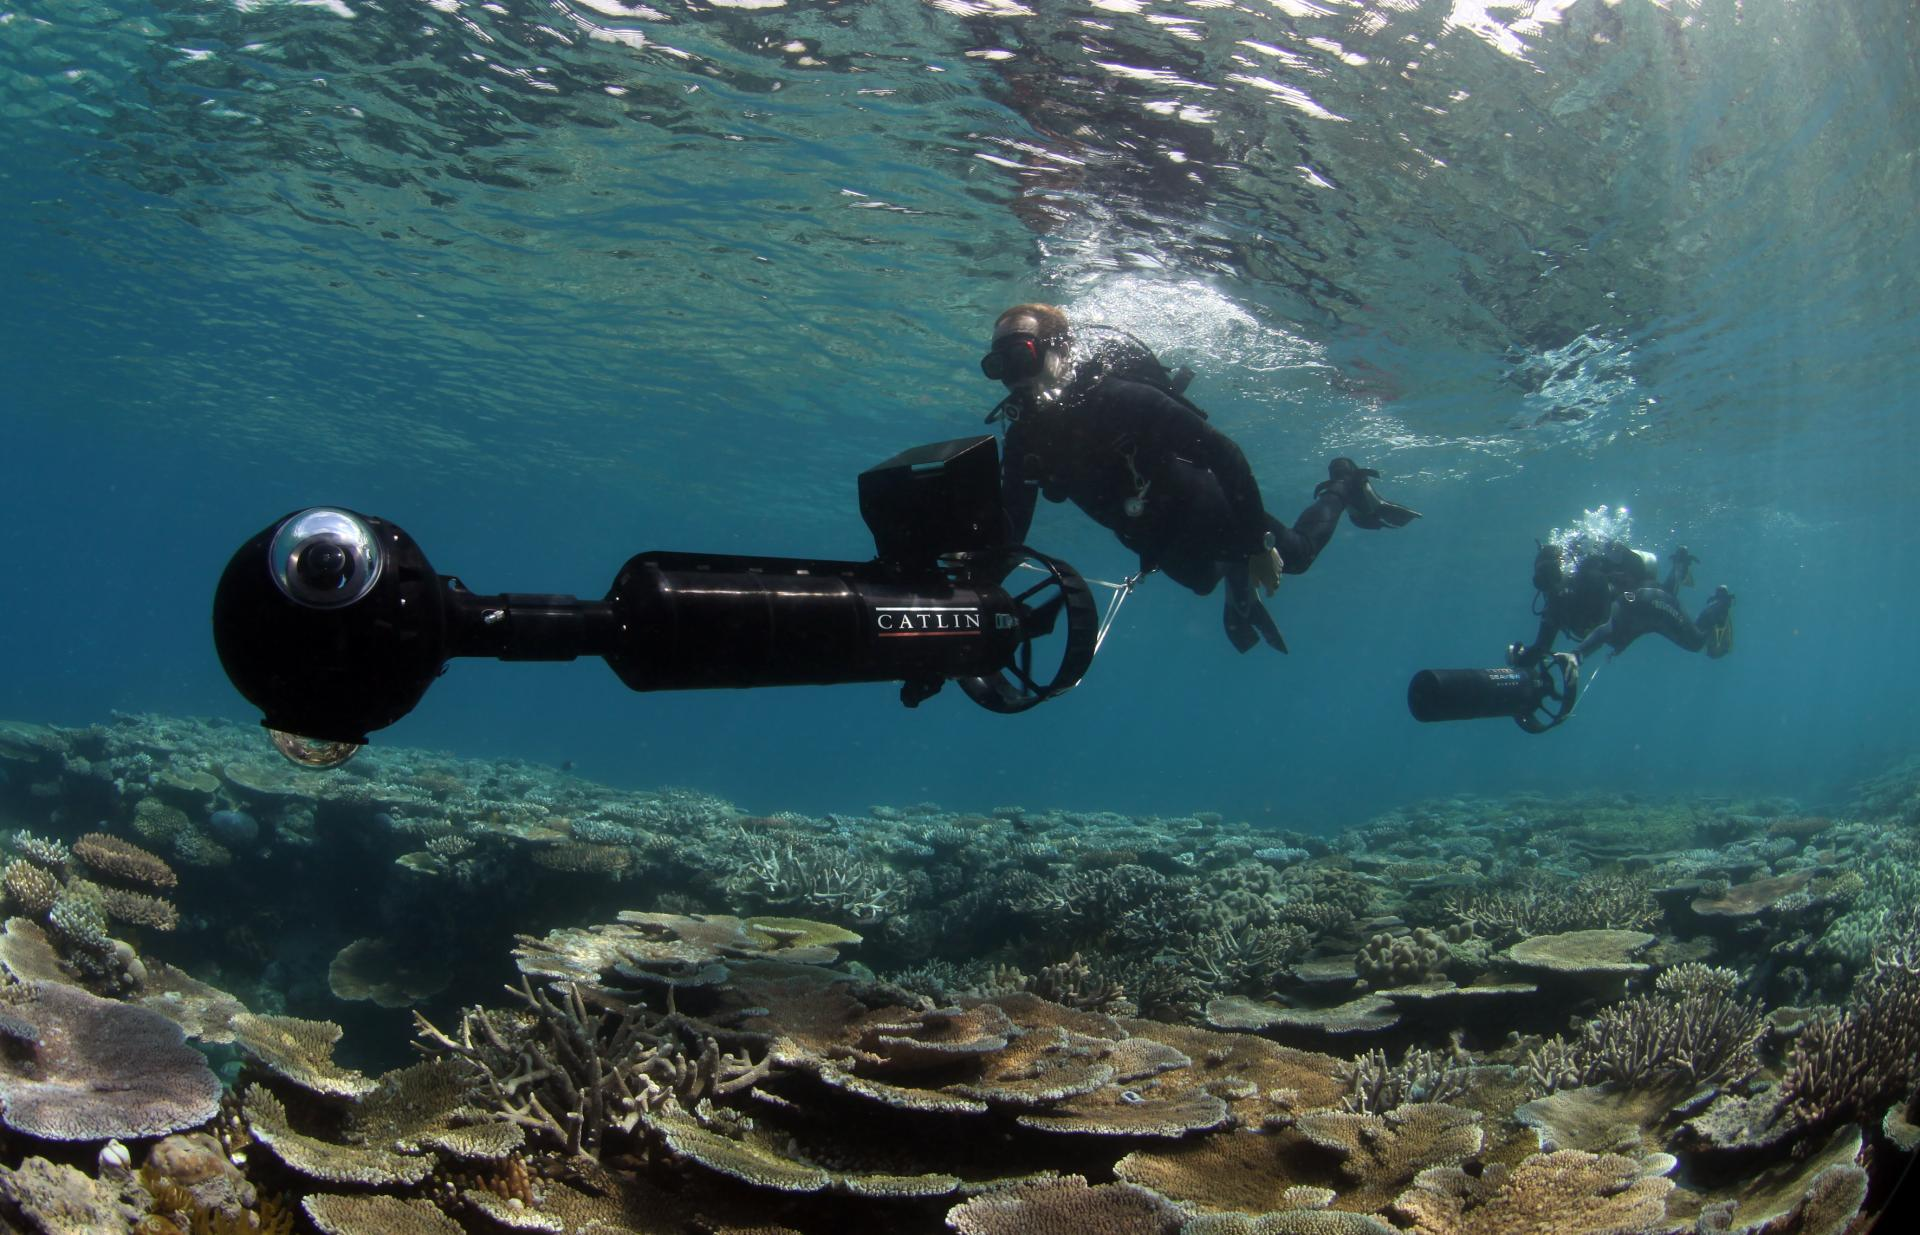
\includegraphics[width = 0.8\textwidth]{SVII.jpg}
                      \caption{{\footnotesize A diver pushing the SVII scooter during a survey of the Great Barrier reef\footnotemark  \copyright XL Catlin Seaview Survey}}
                  \end{figure}

                \end{column}
              \end{columns}
              \footnotetext{\emph{Scaling up ecological measurements of coral reefs using \newline semi-automated field image collection and analysis} \newline Manuel Gonzalez - Rivero et al. 2016}
            \end{frame}

            \begin{frame}
                \begin{figure}
                    \centering
                    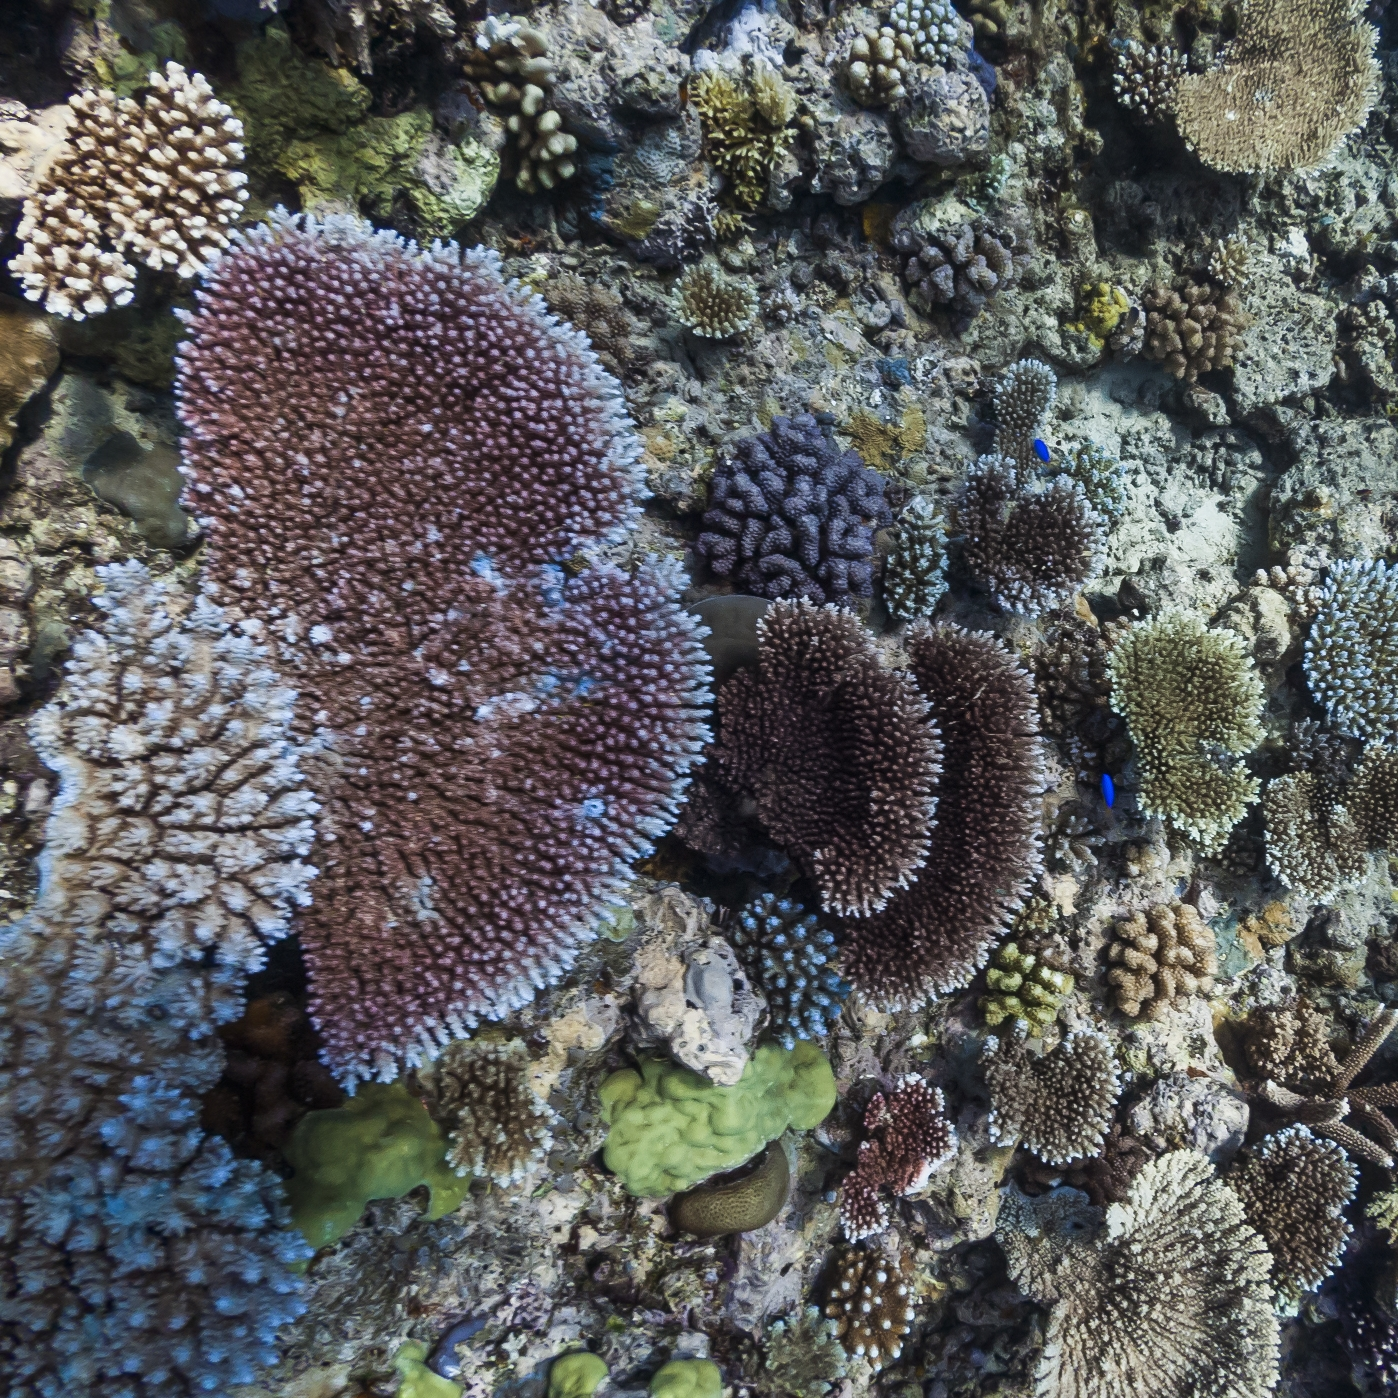
\includegraphics[width = 0.5\textwidth]{coral.jpg}
                    \caption{An example image from a survey of the Great Barrier Reef. Images like this, along with the data, are available on the XL Catlin Global Reef Record\footnotemark. \footnotetext{The Ocean Agency. \emph{Global Reef Record} (2017) URL: \url{http://globalreefrecord.org/data}}}
                \end{figure}
            \end{frame}

          \subsection{Image Annotation}
              \begin{frame}{Neural Network for Image Annotations}
                \begin{itemize}
                  \item Previously a time consuming, manual task (potentially 3 decades of work for the CSS images)
                  \item An automatic point-annotation method is now used based on machine learning algorithms\footnotemark. \footnotetext{O. Beijbom et al. \emph{Towards Automated Annotation of Benthic \newline Survey Images: Variability of Human Experts and Operational \newline Modes of Automation} (2015)}
                  \item Colour and texture of images are used as descriptors for label categories
                  \item Coverage estimates are uploading within a week of collection
                \end{itemize}
              \end{frame}

              \begin{frame}
                  \begin{figure}
                      \centering
                      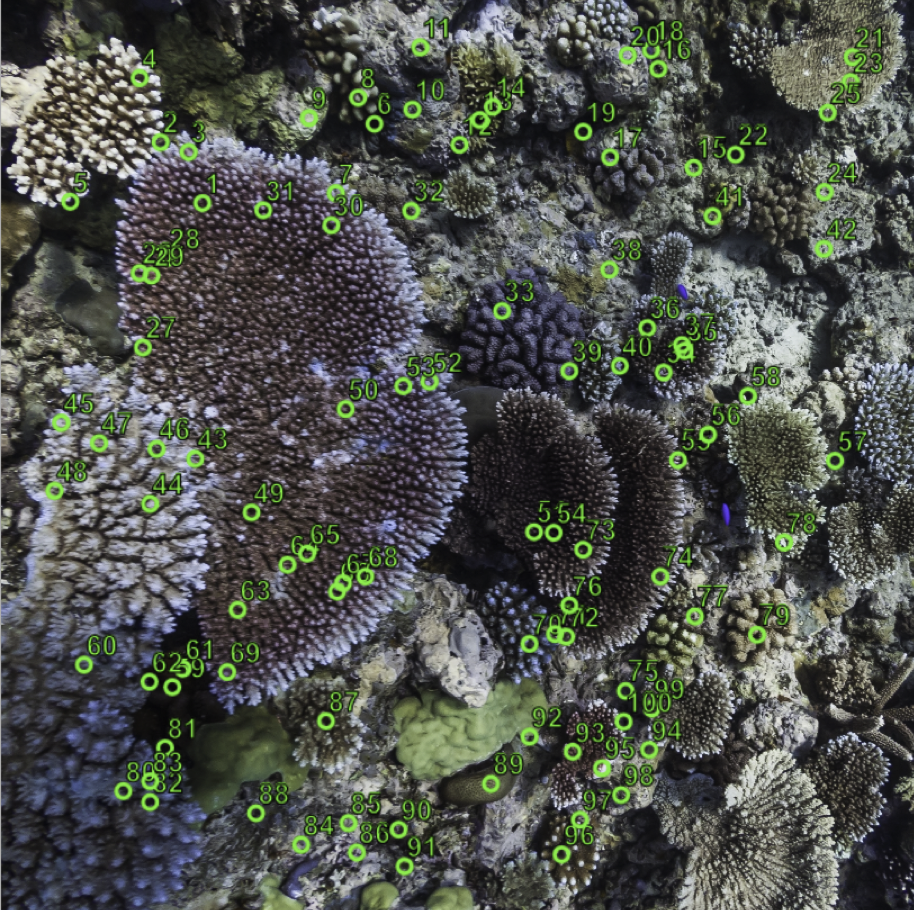
\includegraphics[width = 0.5\textwidth]{coral_points.jpg}
                      \caption{The same image from earlier showing the points used for annotation}
                  \end{figure}
              \end{frame}

    \section{The Need}
        \subsection{Efficient SummaRisation}
            \begin{frame}{The Next Stage}
                \begin{itemize}
                  \item Fast data collection $\rightarrow$ fast annotation $\rightarrow$ bottle neck in processing
                  \item Data stored using MySQL database, allowing for easy integration with RStudio\footnotemark \footnotetext{RMySQL, Joroen Oooms et al. 2017}
                  \item Introducing Rmarkdown\footnotemark \footnotetext{Rmarkdown, JJ Allaire et al. 2017}
                  \item rmarkdown provides a solution for quick/consistent exploratory analysis of the data in a report format
                  \item Visualisations\footnotemark! \footnotetext{Tidyverse, Hadley Wickham 2017}
                \end{itemize}
            \end{frame}


      \section{New Challenges}
        \subsection{Contextual Challenges}
            \begin{frame}{Contextual Challenges}
                \begin{itemize}
                    \item Usability for non R users
                    \item Meaningful visualisations
                    \begin{itemize}
                       \item They need to be useful for more than just the researchers; local government and others in charge of marine protection need to get some value
                       \item Comparisons to literature
                       \item Many label groups, and spatial scales in the dataset
                    \end{itemize}
                \end{itemize}
              \end{frame}

        \subsection{Data Challenges}
            \begin{frame}{Data Challenges - Structure}
                \begin{center}
                  \begin{table}
                    \begin{tabular}{l r r r}
                      Sub-region            &   Reef Count      &   Transect Count      &   Image Count           \\ \hline
                      Cairns-Cooktown       &   13              &   43                  &   87631                 \\
                      Coral Sea             &   3               &   32                  &   23573                 \\
                      Far Northern          &   12              &   33                  &   68367                 \\
                      Mackay-Capricorn      &   4               &   12                  &   14151                 \\
                      Townsville-Whitsunday &   4               &   10                  &   5722                  \\
                      Total                 &   36              &   130                 &   {\color{red}{199444}} \\
                    \end{tabular}
                      \label{tab:GBRSummary}
                      \caption{A summary of the various spatial scales within just one region, the Great Barrier Reef. This structure is consistent across all 5 regions.}
                  \end{table}
                \end{center}
            \end{frame}

            \begin{frame}{Data Challenges - Labels}
                \begin{itemize}
                  \item Benthic labels describe the community benthic category
                  \item Global labels describe morphological categories
                  \item Each region has 5 functional groups
                  \begin{itemize}
                    \item Hard corals, soft corals
                    \item Algae
                    \item Other invertibrates, other
                  \end{itemize}
                \end{itemize}

              \begin{center}
                  \begin{table}
                      \begin{tabular}{l r r r}
                          Region                &   Benthic Labels         &   Global Labels   \\ \hline
                          GBR                   &   27                     &   13              \\
                          Indian Ocean          &   49                     &   17              \\
                          Caribbean             &   67                     &   16              \\
                          Southeast Asia        &   71                     &   17              \\
                          Pacific               &   40                     &   12              \\
                      \end{tabular}
                  \end{table}
              \end{center}
            \end{frame}

      \section{Solutions}
          \subsection{Dynamic Plotting Environments}

              \begin{frame}{The Visualisations and Dynamic Plotting}
                Several Challenges
                  \begin{itemize}
                    \item Needed at multiple spatial scales and to be reproducible
                    \item Differing label sets among regions
                    \item Single survey regions
                  \end{itemize}

                  \medskip

                Several Solutions
                  \begin{itemize}
                    \item Variable figure heights
                    \item Lots and lots of data cleaning and aggregation
                  \end{itemize}
              \end{frame}

              \begin{frame}{Dynamic Plotting}
                \begin{itemize}
                  \item The code wrapper in the rmarkdown source script allows you to set a variable to the figure heights and widths
                \end{itemize}

                \begin{figure}
                    \centering
                    \includegraphics[width = \textwidth]{DynamicPlot.png}
                    \caption{Plot wrapper with an exmaple of the figure height addjustment according to the number of plot facets. Also shows here is a boolean variable for evaluation of the code segment. }
                \end{figure}
              \end{frame}

              \begin{frame}{Reef Scale Visualisations}
                \begin{figure}
                    \centering
                    \includegraphics[width = \textwidth]{ReefVis.png}
                    \caption{An example visualisation of only 3 of the 36 GBR reefs. This plot is created at the functional group scale. Note that the x axis is year, and the y axis is percentage coverage over the reef in question. }
                \end{figure}
             \end{frame}

             \begin{frame}{Reef Scale Visualisations}
                \begin{figure}
                    \centering
                    \includegraphics[width = \textwidth]{ReefVisSingle.png}
                    \caption{An example of the reef scale visualisaton for the reefs only surveyed once. Coverage here is represented in the same way as the previous plot, giving a percentage coverage for each basic functional group.}
                \end{figure}
             \end{frame}

             % \begin{frame}{Subregion Visualisations}
             %    \begin{figure}
             %        \centering
             %        \includegraphics[width = 0.55\textwidth]{SubregionVis.png}
             %        \caption{An example of subregion scale visualisations}
             %    \end{figure}
             % \end{frame}

             \begin{frame}{Change at the Transect Scale}
               \begin{columns}[T]
                 \begin{column}{0.48\textwidth}
                   \centering
                    \begin{figure}
                        \centering
                        \includegraphics[width = \textwidth]{PlotChange.png}
                   \end{figure}
                 \end{column}
                 \begin{column}{0.48\textwidth}
                   \centering
                    \begin{itemize}
                      \item Extra challenges that arise from survey design
                      \item Visualised at the global label level
                      \item Investigate change only over consecutive survey years
                    \end{itemize}
                 \end{column}
              \end{columns}
             \end{frame}

             \subsection{Interactive Maps using Leaflet}
                 \begin{frame}{Leaflet}

                    Using Leaflet\footnotemark \footnotetext{\emph{Leaflet} J. Cheng, B. Karambelkar, Y. Xie 2017} for interactive maps allows for readers to see where exactly the surveys take place. Each transect marker represents a 2km survey region.

                     \begin{figure}
                        \centering
                        \includegraphics[width = 0.55\textwidth]{Leaflet.png}
                        \caption{Disclaimer - this image is not so interactive }
                     \end{figure}
                 \end{frame}


          \subsection{RMySQL and Parameterised Rmarkdown}
              \begin{frame}{Parameterising Rmarkdown Documents and RMySQL}
                RMySQL allows for accessing the database through Rstudio negating the need for an external program
                  \begin{figure}
                    \centering
                    \begin{subfigure}[t]{0.48\textwidth}
                      \centering
                        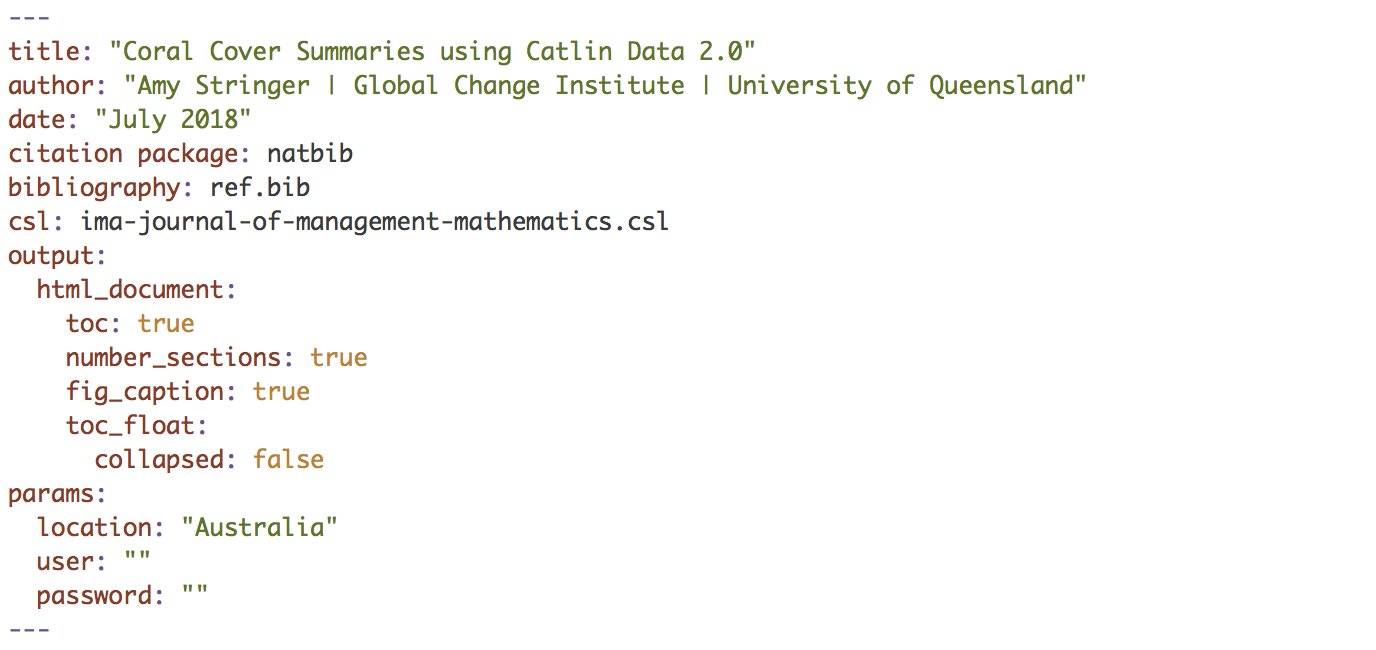
\includegraphics[width = \textwidth]{yaml_header.png}
                        \caption{The header when making use of document parameters. In future, more parameters may be added to simplify the source script, but in the current stages things have been kept simple.}
                        \label{fig:yaml_header}
                    \end{subfigure}\hskip 1em%
                    \begin{subfigure}[t]{0.48\textwidth}
                      \centering
                        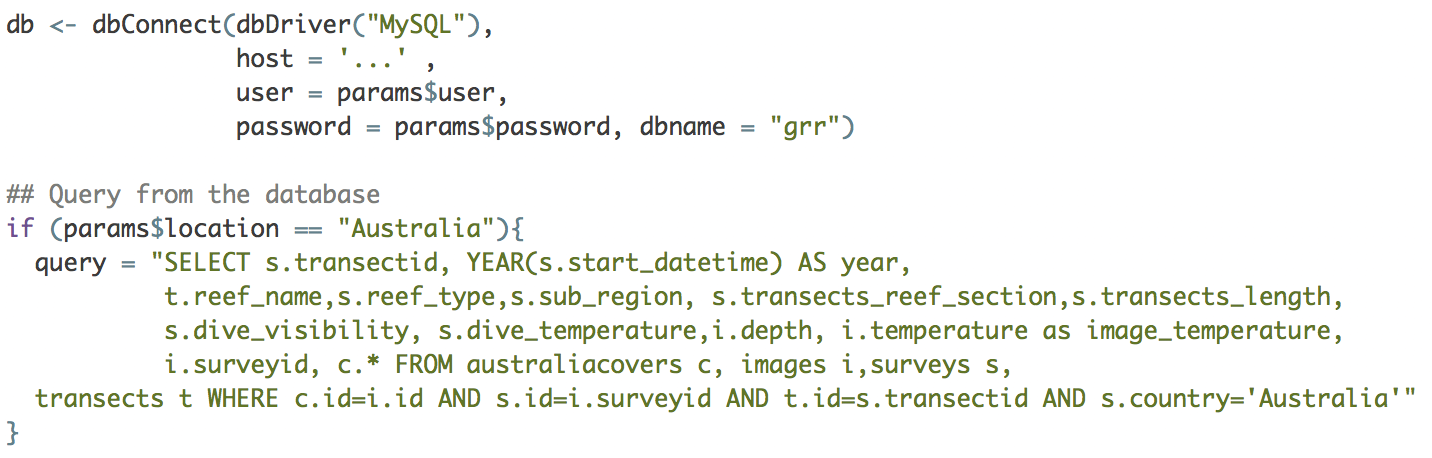
\includegraphics[width = \textwidth]{SQL_connect.png}
                        \caption{Working example accessing the database with the document input parameters. The use of RMySQL allows for connection to the database and extraction of data within the Rmarkdown source script.}
                        \label{fig:SQL_connect}
                    \end{subfigure}
                  \end{figure}
                \end{frame}

                \begin{frame}{How's the SeRenity?}
                    \begin{figure}
                        \centering
                        \includegraphics[width = \textwidth]{useR.png}
                        \caption{The only bit of code a user needs to deal with to generate up to 25 reports.}
                    \end{figure}

                \end{frame}

          \subsection{Child Documents}
              \begin{frame}{Child Documents for Textual Components}
                  \begin{itemize}
                    \item Introductions and discussions will need to be different across the regions
                    \item Using the parameters of the source we can import a specific introduction file for each desired region
                    \item Child documents allow for easy editing of introductions/methods/discussions, without needing to open the main source document which is overwhelming and complicated
                  \end{itemize}
              \end{frame}

      \section{Future Work}
        \begin{frame}{Future Work}
          \begin{itemize}
            \item Currently this isn't a fully automated process
            \item Talk of linking these reports to a website
            \item Extra parameterisation of the document - perhaps a structure change based on the individual generating the report (e.g. management, research etc)
          \end{itemize}
        \end{frame}



\end{document}
